\chapter{Introduction}%
\label{ch:intro}

In 2012 the Higgs boson was discovered by the ATLAS and CMS collaborations at
the Large Hadron Collider~\cite{DiscoHiggsATLAS, DiscoHiggsCMS}. It was said to
form the last piece of the Standard Model of Particle Physics, a framework that
describes three of the four fundamental forces of nature, described in more
detail in Chapter~\ref{ch:theory}. Despite apparent completeness after the
Higgs discovery, it is known that the theory does not describe gravity, the
fourth of the known fundamental forces of nature. The theory also has other
shortcomings, it cannot explain the presence of dark matter~\cite{DM-ev-sloan,
  DM-ev-nucleosynth, DM-ev-supernova, DM-ev-scaffold, DM-ev-direct,
  DM-ev-strong-lens, DM-ev-candidates, DM-ev-PDG, DM-ev-Zwicky,
  DM-ev-nonbaryonic, DM-ev-particle} or a number of other observed
phenomena~\cite{anom-BD-branching, anom-Dtau-excess, anom-g-2,
  anom-proton-radius, anom-bsll-trans}. So far the model has stood up to all
experimental tests~\cite{EWtests, 1998-SMtests} concerning its own predictions
but there are still parameters of the model that have not been measured. Given
the theory's understood shortcomings, it is hoped that continued scrutiny of the
models predictions will yield unexpected results, perhaps hinting at a new
way forwards in terms of a theory that describes all matter and forces in the
universe or simply exposing further gaps in our knowledge. For this reason it is
more important than ever to study in detail the most recently discovered piece
of the model, the Higgs boson.

This work focuses on studying a specific production mechanism and decay mode of
the Higgs boson, specifically a vector boson associated Higgs boson decaying to
two bottom quarks, denoted \VHbb. This decay mode is of importance as it is
currently the only decay mode of the Higgs decaying to quarks that has been
observed~\cite{vhbb-obs}. A summary of the full spectrum of production
mechanisms and decay modes of the Higgs will be given in
Chapter~\ref{ch:theory}.

The data used to study this decay mode was collected using the ATLAS detector by
members of the ATLAS collaboration. The collection of this data is only made
possible by their hard work and by the hard work of everyone working on the
Large Hadron Collider at CERN.

A rough blueprint of this analysis is shown in figure~\ref{fig:roadmap}.%
\begin{figure}[ht]
  \centering
  %Define block styles
  \tikzstyle{decision} = [diamond, draw, fill=blue!20, 
  text width=4.5em, text badly centered, node distance=3cm, inner sep=0pt]
  \tikzstyle{block} = [rectangle, draw, fill=blue!20, text width=12em, text
  centered, rounded corners, minimum height=3em]
  \tikzstyle{line} = [draw, -latex']
  \tikzstyle{cloud} = [fill=none, minimum
  height=2em]
  
    
  \begin{tikzpicture}[node distance = 2cm, auto]
    % Place nodes
    \node[cloud] (root) {};
    \node[cloud, left =of root, align=left] (theory) {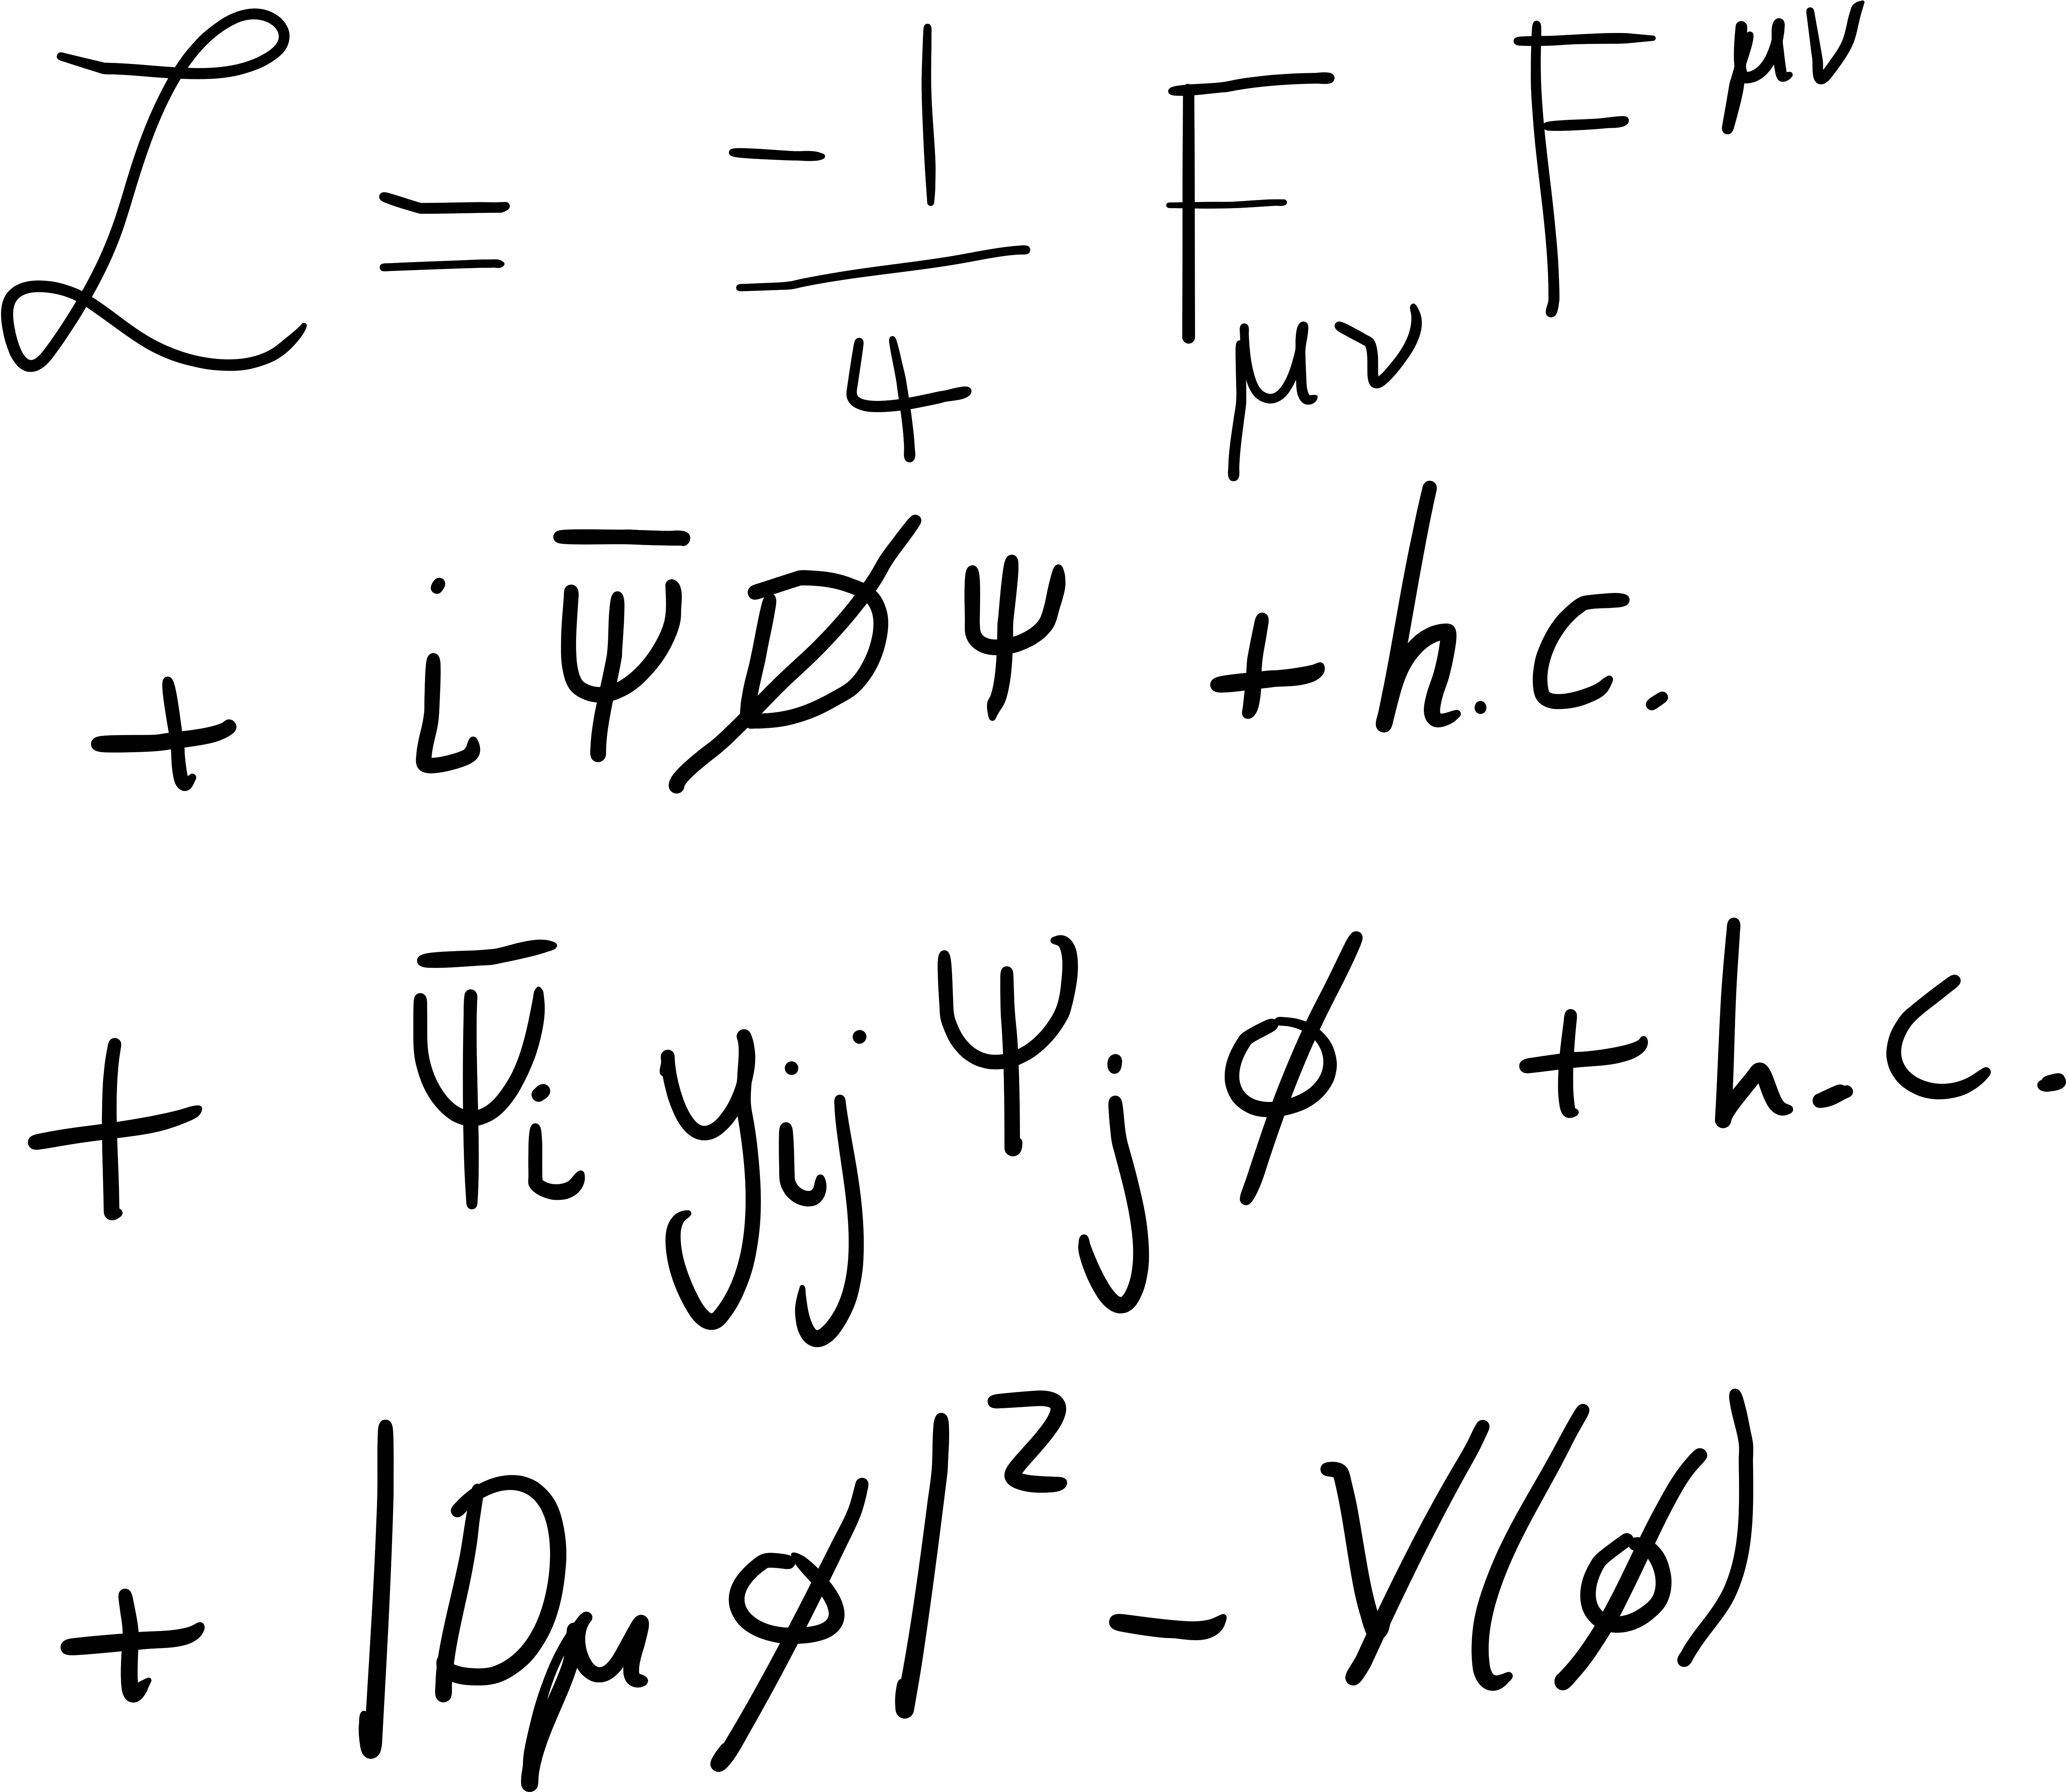
\includegraphics[width=.25\textwidth]{hand_written_lagrangian-1} \\Theory};
    
    \node [cloud, right=of root, align=left] (detector)  {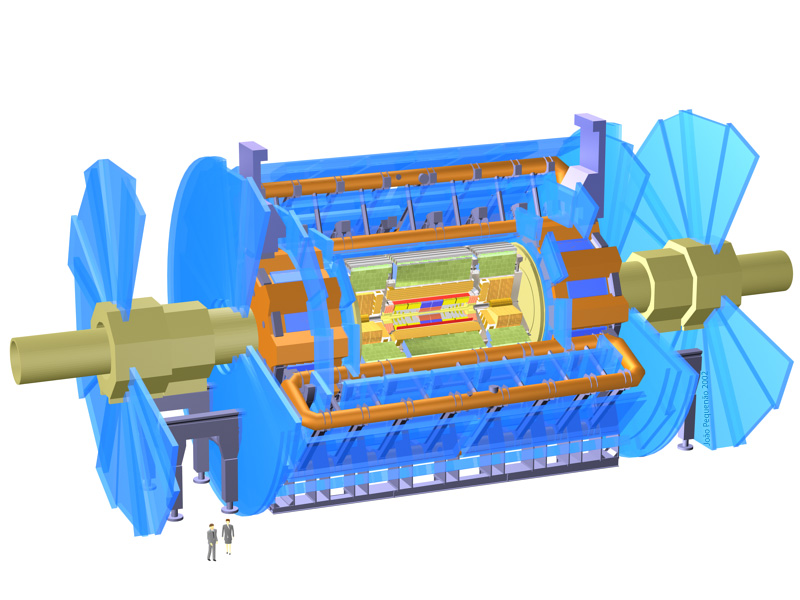
\includegraphics[width=.25\textwidth]{atlas_big} \\Detector};

    \node [cloud, below=of root, align=left] (recon)  {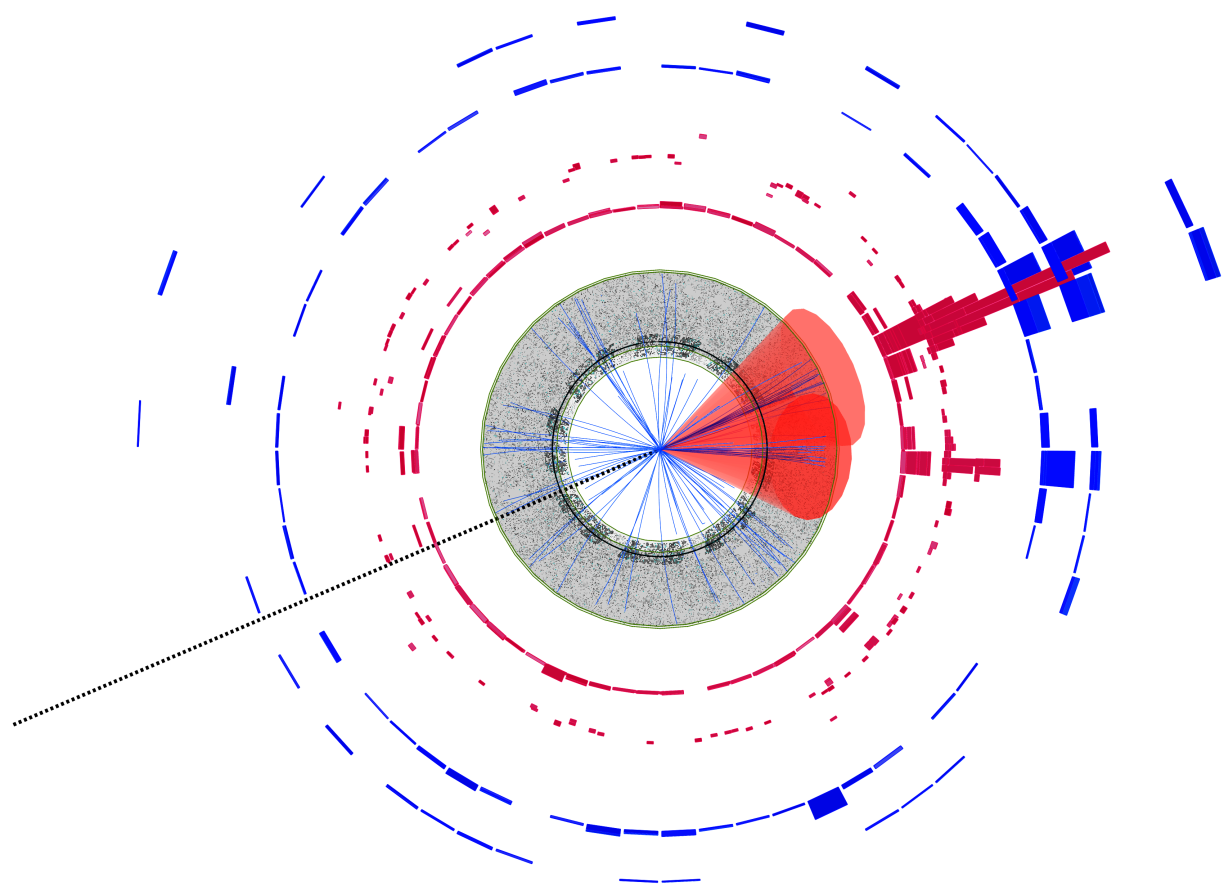
\includegraphics[width=.25\textwidth]{Event_Display_inv} \\Reconstruction};

    \node [cloud, below=of recon] (ghost1) {};
    
    \node [cloud, left=of ghost1, align=left] (modelling)  {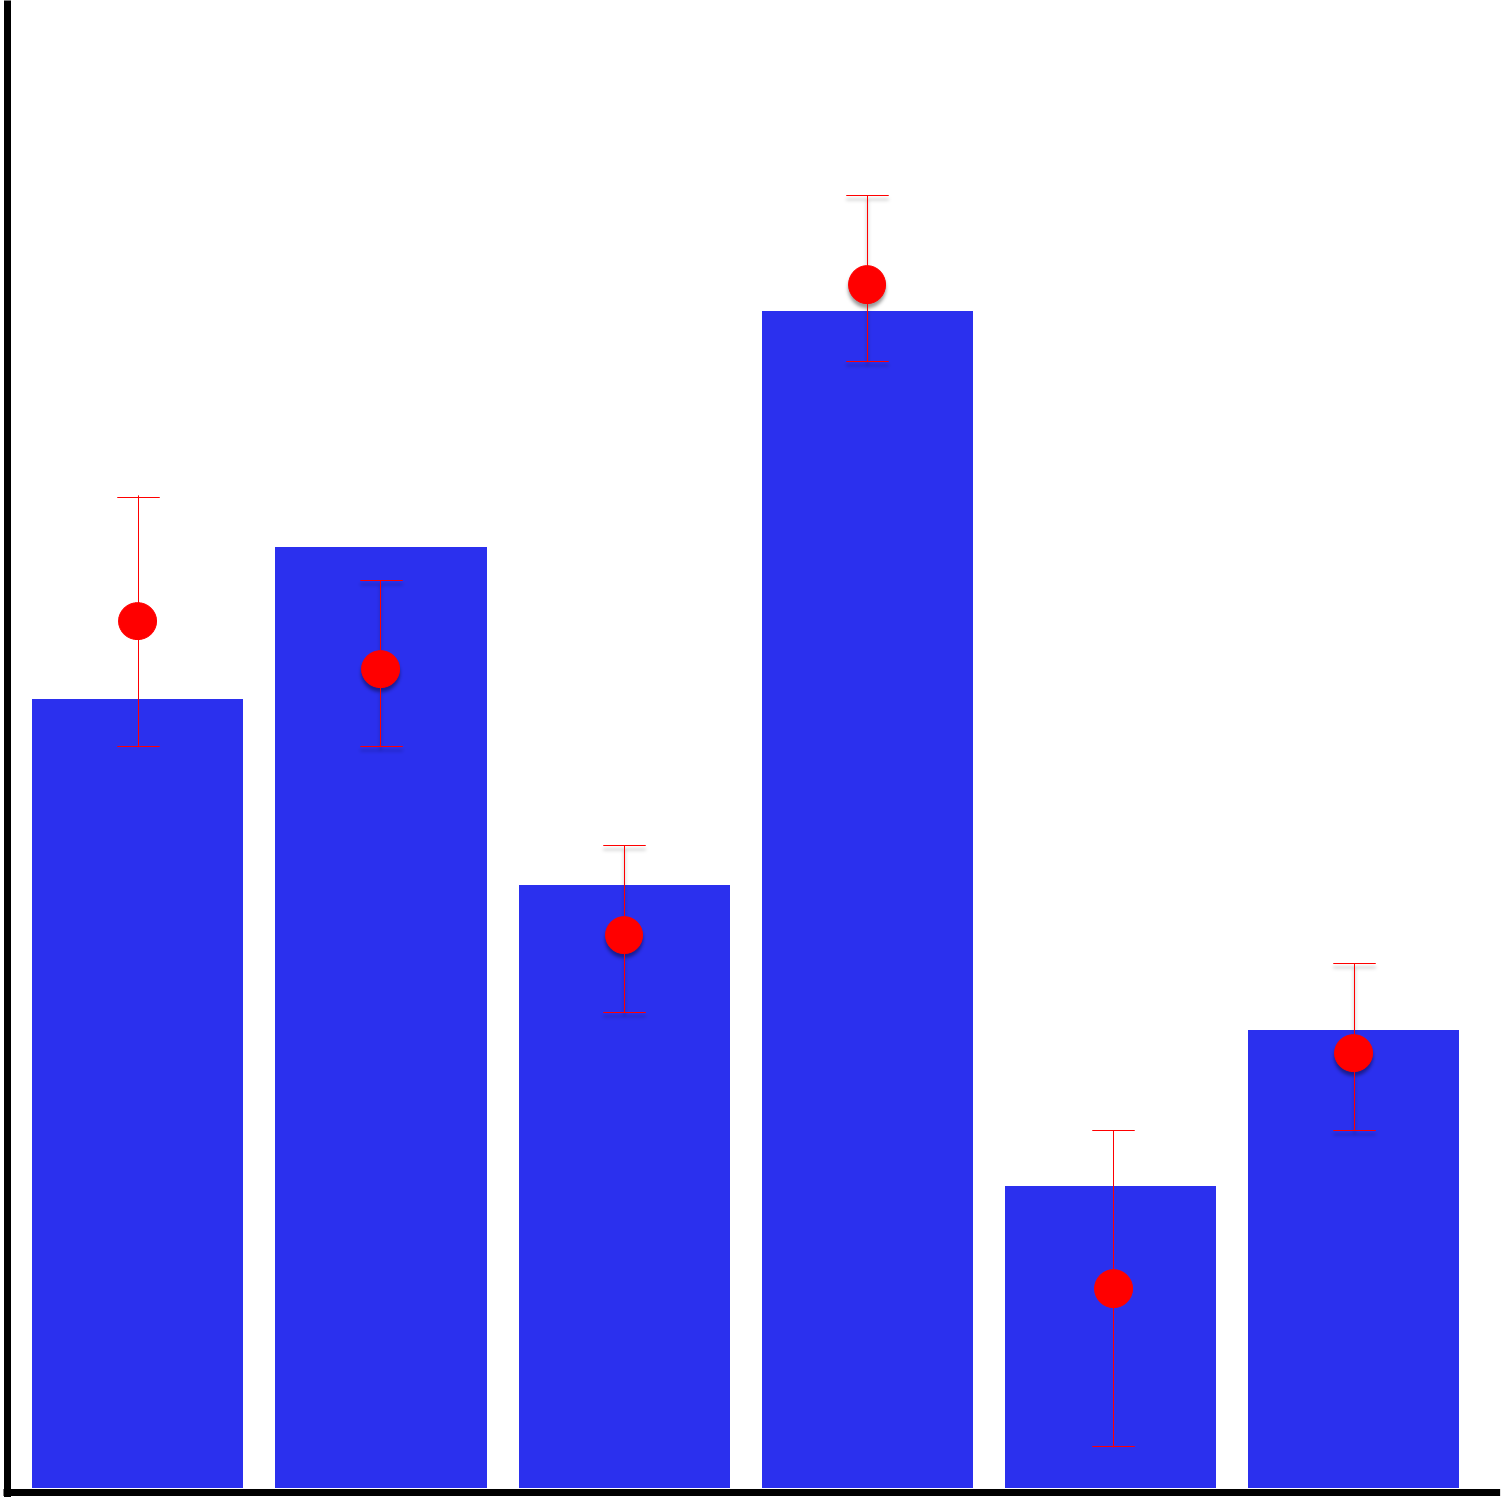
\includegraphics[width=.25\textwidth]{generic_data_mc} \\Modelling};

    \node [cloud, right=of ghost1, align=left] (mva)  {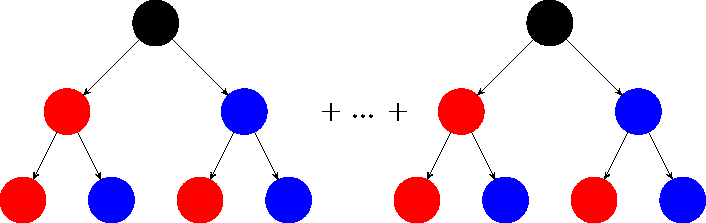
\includegraphics[width=.25\textwidth]{mini-bdt} \\Categorisation};

    \node [cloud, below=of ghost1, align=left] (plf)  {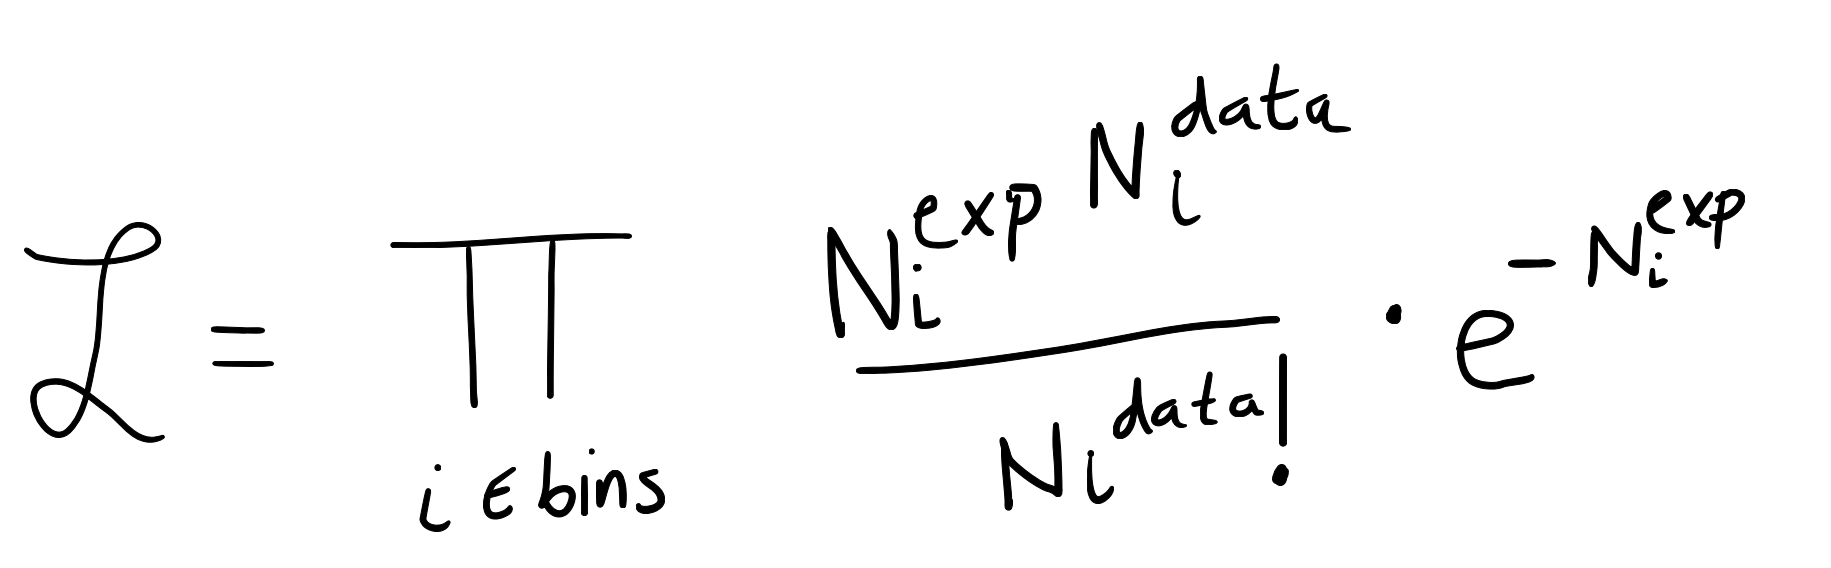
\includegraphics[width=.45\textwidth]{plf_handwritten} \\Profile-Likelihood Fit};

    \node [cloud, below=of plf, align=left] (results)  {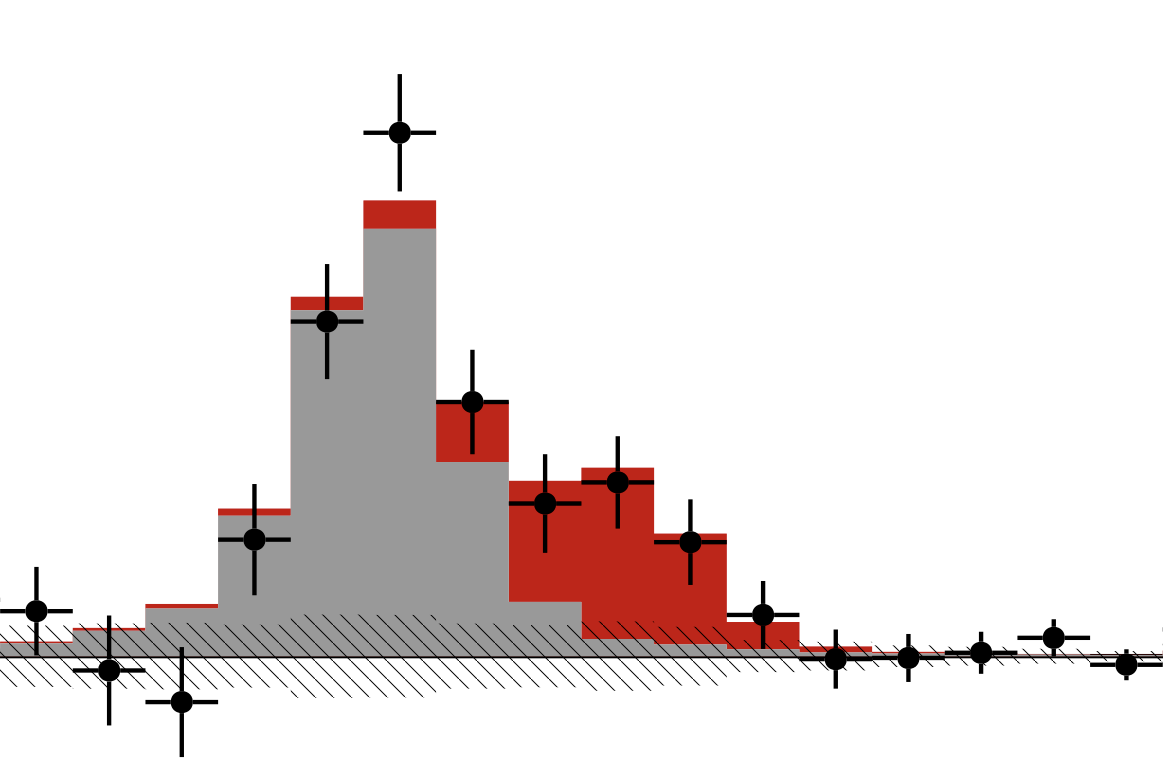
\includegraphics[width=.25\textwidth]{hbb_plot} \\Results \& Conclusions};
    
    % Draw edges 
    \path [line] (theory) -- (detector);

    \path [line] (detector) -- (recon);

    \path [line] (detector) to [out=200,in=70] (modelling);

    \path [line] (recon) -- (modelling);

    \path [line] (recon) -- (mva);

    \path [line] (mva) -- (plf);

    \path [line] (modelling) -- (plf);

    \path [line] (plf) -- (results);
    
  \end{tikzpicture}
  \caption[A roadmap of the analysis.]{A flow chart showing the roadmap of the \VHbb\ analysis and of this thesis.}
  \label{fig:roadmap}
\end{figure}
The blueprint starts with the theory of the Standard Model of Particle Physics,
described in chapter~\ref{ch:theory}. The theory's predictions inform the
design of the ATLAS detector which is detailed in chapter~\ref{ch:detector}.
Furthermore, the theory aids the choice of particles to collide, which events to
analyse, and allows us to generate predictions of what should happen in the
collisions. Chapter~\ref{ch:ml} gives an overview of two machine learning
algorithms that are used throughout the analysis. Events must be reconstructed
before they can be analysed, a selection process is used on the reconstructed
objects to filter events not relevant to the analysis. The reconstruction and
selection process is described in chapter~\ref{ch:recon}. Events in data must
be categorised into those that are signal-like and those that are
background-like in order to extract the most signal sensitivity from the
analysis. This is achieved with a number of strategies including a multi-variate
algorithm which is trained on the simulations. This categorisation process is
described in chapter~\ref{ch:strategy}, along with the overall analysis
strategy. A choice is made of simulated events that well model the data.
Considering the modelling, the theory and the shortcomings of the detector a set
of systematic errors are estimated, these are detailed in~\ref{ch:systematics}.
With the events categorised and the systematic errors on the counts in category
estimated, these counts serve as inputs to a profile-likelihood fit. Several fit
models exist to serve a number of purposes, the fit models are described in
chapter~\ref{ch:fit-models}. The results of the analysis are shown in
chapter~\ref{ch:results} and conclusions are drawn in
chapter~\ref{ch:conclusion}.


My contributions to the \VHbb\ analysis published in 2021 have been numerous and
spanned a number of different areas of the analysis.

My largest contribution was the derivation of new estimates of background
modelling uncertainties. This includes deriving new shape uncertainty estimates
for the $Z+$jets background in the 0 and 2 lepton channels which use a method
which includes a number of improvements over the previous analysis (explained in
detail in chapter~\ref{ch:systematics}). I also calculated estimates of
uncertainties arising due to differences in the flavour composition and yields
in given analysis regions between simulation and data for the $Z+$jets and top
backgrounds. I helped to develop and test code which performs a
multi-dimensional re-weighting of one dataset to another. This technique has
been used to estimate uncertainties of the top backgrounds and $W+$jets
backgrounds in the 1 lepton channel.

My next largest contribution was to studying the profile likelihood fit that
outputs the final analysis results. During key milestones of the analysis it is
often necessary to compare the blinded results of the fit to study the behaviour
of nuisance parameters and how they are pulled, constrained and correlated with
one another. I performed many of these comparisons paying close attention to the
nuisance parameters relating to the aforementioned estimates on background
modelling uncertainties. After approval was granted to unblind the analysis I
was also responsible for running the final fit for the diboson measurement which
serves as a cross-check of the all of the analysis methodology used for the
Higgs measurement.

Finally I have also made contributions to the general running of the analysis.
These including training the classification algorithm which provides the final
discriminating metric upon which the profile-likelihood fit is performed,
helping to maintain the analysis framework (which is also used by many other
ATLAS analyses) and participating in regular meetings with the analysis team
where ideas are discussed and the general analysis direction is decided.
